\documentclass{standalone}
\usepackage{tikz}
\usetikzlibrary{patterns, positioning}

\begin{document}
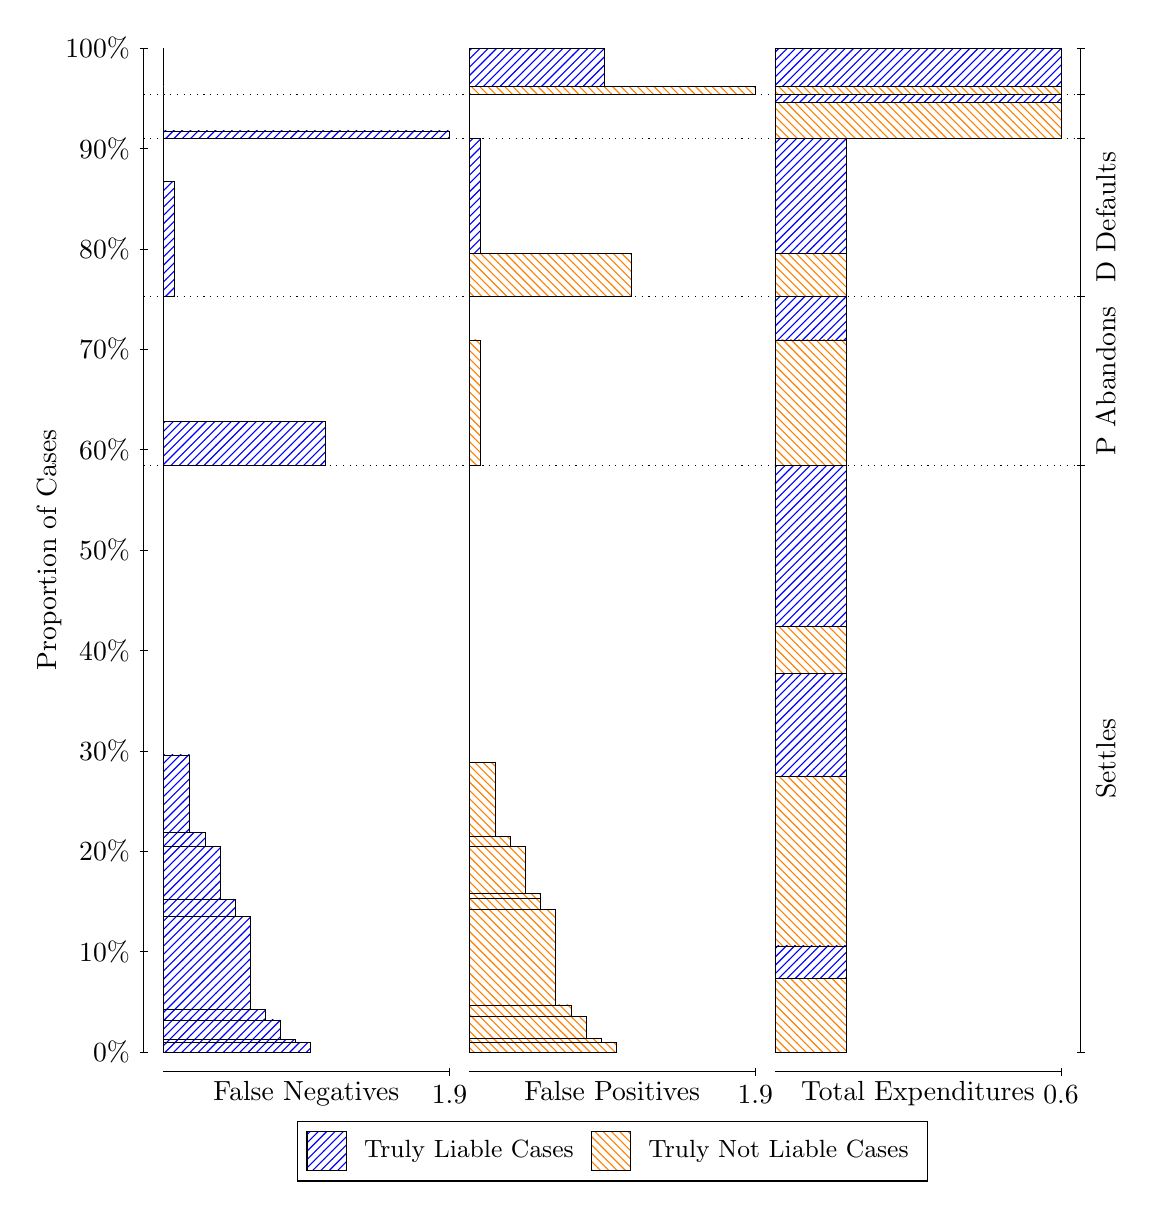
\begin{tikzpicture}
\draw[black, very thin] (1.5,1.75) -- (1.5,14.5);
\node[rotate=90, anchor=center] at (0.3, 8.125) {Proportion of Cases};
\draw[black, very thin] (1.45,1.75) -- (1.55,1.75);
\node[anchor=east] at (1.45, 1.75) {0\%};
\draw[black, very thin] (1.45,3.025) -- (1.55,3.025);
\node[anchor=east] at (1.45, 3.025) {10\%};
\draw[black, very thin] (1.45,4.3) -- (1.55,4.3);
\node[anchor=east] at (1.45, 4.3) {20\%};
\draw[black, very thin] (1.45,5.575) -- (1.55,5.575);
\node[anchor=east] at (1.45, 5.575) {30\%};
\draw[black, very thin] (1.45,6.85) -- (1.55,6.85);
\node[anchor=east] at (1.45, 6.85) {40\%};
\draw[black, very thin] (1.45,8.125) -- (1.55,8.125);
\node[anchor=east] at (1.45, 8.125) {50\%};
\draw[black, very thin] (1.45,9.4) -- (1.55,9.4);
\node[anchor=east] at (1.45, 9.4) {60\%};
\draw[black, very thin] (1.45,10.675) -- (1.55,10.675);
\node[anchor=east] at (1.45, 10.675) {70\%};
\draw[black, very thin] (1.45,11.95) -- (1.55,11.95);
\node[anchor=east] at (1.45, 11.95) {80\%};
\draw[black, very thin] (1.45,13.225) -- (1.55,13.225);
\node[anchor=east] at (1.45, 13.225) {90\%};
\draw[black, very thin] (1.45,14.5) -- (1.55,14.5);
\node[anchor=east] at (1.45, 14.5) {100\%};

\draw[black, very thin] (13.4,1.75) -- (13.4,14.5);
\draw[black, very thin] (13.35,1.75) -- (13.45,1.75);
\node[anchor=west] at (13.35, 1.75) {};
\draw[black, very thin] (13.35,9.1995) -- (13.45,9.1995);
\node[anchor=west] at (13.35, 9.1995) {};
\draw[black, very thin] (13.35,11.35) -- (13.45,11.35);
\node[anchor=west] at (13.35, 11.35) {};
\draw[black, very thin] (13.35,13.349) -- (13.45,13.349);
\node[anchor=west] at (13.35, 13.349) {};
\draw[black, very thin] (13.35,13.911) -- (13.45,13.911);
\node[anchor=west] at (13.35, 13.911) {};
\draw[black, very thin] (13.35,14.5) -- (13.45,14.5);
\node[anchor=west] at (13.35, 14.5) {};

\draw[black, very thin, pattern color=blue, pattern=north east lines] (1.75,1.75) rectangle (3.6145,1.8758);
\draw[black, very thin, pattern color=blue, pattern=north east lines] (1.75,1.8758) rectangle (3.4232,1.9069);
\draw[black, very thin, pattern color=blue, pattern=north east lines] (1.75,1.9069) rectangle (3.232,2.1589);
\draw[black, very thin, pattern color=blue, pattern=north east lines] (1.75,2.1589) rectangle (3.0408,2.2919);
\draw[black, very thin, pattern color=blue, pattern=north east lines] (1.75,2.2919) rectangle (2.8496,3.4742);
\draw[black, very thin, pattern color=blue, pattern=north east lines] (1.75,3.4742) rectangle (2.6583,3.6845);
\draw[black, very thin, pattern color=blue, pattern=north east lines] (1.75,3.6845) rectangle (2.4671,4.3601);
\draw[black, very thin, pattern color=blue, pattern=north east lines] (1.75,4.3601) rectangle (2.2759,4.5348);
\draw[black, very thin, pattern color=blue, pattern=north east lines] (1.75,4.5348) rectangle (2.0846,5.5219);
\draw[black, very thin, pattern color=orange, pattern=north west lines] (1.75,5.5219) rectangle (1.75,9.1995);
\draw[black, very thin, pattern color=blue, pattern=north east lines] (1.75,9.1995) rectangle (3.8057,9.7569);
\draw[black, very thin, pattern color=orange, pattern=north west lines] (1.75,9.7569) rectangle (1.75,11.35);
\draw[black, very thin, pattern color=blue, pattern=north east lines] (1.75,11.35) rectangle (1.8934,12.807);
\draw[black, very thin, pattern color=orange, pattern=north west lines] (1.75,12.807) rectangle (1.75,13.349);
\draw[black, very thin, pattern color=blue, pattern=north east lines] (1.75,13.349) rectangle (5.3833,13.448);
\draw[black, very thin, pattern color=orange, pattern=north west lines] (1.75,13.448) rectangle (1.75,13.911);
\draw[black, very thin, pattern color=orange, pattern=north west lines] (1.75,13.911) rectangle (1.75,14.01);
\draw[black, very thin, pattern color=blue, pattern=north east lines] (1.75,14.01) rectangle (1.75,14.5);
\draw[black, very thin, pattern color=orange, pattern=north west lines] (5.6333,1.75) rectangle (7.4978,1.8744);
\draw[black, very thin, pattern color=orange, pattern=north west lines] (5.6333,1.8744) rectangle (7.3066,1.9207);
\draw[black, very thin, pattern color=orange, pattern=north west lines] (5.6333,1.9207) rectangle (7.1154,2.2064);
\draw[black, very thin, pattern color=orange, pattern=north west lines] (5.6333,2.2064) rectangle (6.9241,2.3485);
\draw[black, very thin, pattern color=orange, pattern=north west lines] (5.6333,2.3485) rectangle (6.7329,3.5606);
\draw[black, very thin, pattern color=orange, pattern=north west lines] (5.6333,3.5606) rectangle (6.5417,3.6973);
\draw[black, very thin, pattern color=orange, pattern=north west lines] (5.6333,3.6973) rectangle (6.5417,3.7604);
\draw[black, very thin, pattern color=orange, pattern=north west lines] (5.6333,3.7604) rectangle (6.3504,4.3654);
\draw[black, very thin, pattern color=orange, pattern=north west lines] (5.6333,4.3654) rectangle (6.1592,4.4923);
\draw[black, very thin, pattern color=orange, pattern=north west lines] (5.6333,4.4923) rectangle (5.968,5.4276);
\draw[black, very thin, pattern color=blue, pattern=north east lines] (5.6333,5.4276) rectangle (5.6333,9.1995);
\draw[black, very thin, pattern color=orange, pattern=north west lines] (5.6333,9.1995) rectangle (5.7768,10.793);
\draw[black, very thin, pattern color=blue, pattern=north east lines] (5.6333,10.793) rectangle (5.6333,11.35);
\draw[black, very thin, pattern color=orange, pattern=north west lines] (5.6333,11.35) rectangle (7.689,11.892);
\draw[black, very thin, pattern color=blue, pattern=north east lines] (5.6333,11.892) rectangle (5.7768,13.349);
\draw[black, very thin, pattern color=orange, pattern=north west lines] (5.6333,13.349) rectangle (5.6333,13.812);
\draw[black, very thin, pattern color=blue, pattern=north east lines] (5.6333,13.812) rectangle (5.6333,13.911);
\draw[black, very thin, pattern color=orange, pattern=north west lines] (5.6333,13.911) rectangle (9.2667,14.01);
\draw[black, very thin, pattern color=blue, pattern=north east lines] (5.6333,14.01) rectangle (7.3544,14.5);
\draw[black, very thin, pattern color=orange, pattern=north west lines] (9.5167,1.75) rectangle (10.425,2.6817);
\draw[black, very thin, pattern color=blue, pattern=north east lines] (9.5167,2.6817) rectangle (10.425,3.0978);
\draw[black, very thin, pattern color=orange, pattern=north west lines] (9.5167,3.0978) rectangle (10.425,5.2452);
\draw[black, very thin, pattern color=blue, pattern=north east lines] (9.5167,5.2452) rectangle (10.425,6.5533);
\draw[black, very thin, pattern color=orange, pattern=north west lines] (9.5167,6.5533) rectangle (10.425,7.1518);
\draw[black, very thin, pattern color=blue, pattern=north east lines] (9.5167,7.1518) rectangle (10.425,9.1995);
\draw[black, very thin, pattern color=orange, pattern=north west lines] (9.5167,9.1995) rectangle (10.425,10.793);
\draw[black, very thin, pattern color=blue, pattern=north east lines] (9.5167,10.793) rectangle (10.425,11.35);
\draw[black, very thin, pattern color=orange, pattern=north west lines] (9.5167,11.35) rectangle (10.425,11.892);
\draw[black, very thin, pattern color=blue, pattern=north east lines] (9.5167,11.892) rectangle (10.425,13.349);
\draw[black, very thin, pattern color=orange, pattern=north west lines] (9.5167,13.349) rectangle (13.15,13.812);
\draw[black, very thin, pattern color=blue, pattern=north east lines] (9.5167,13.812) rectangle (13.15,13.911);
\draw[black, very thin, pattern color=orange, pattern=north west lines] (9.5167,13.911) rectangle (13.15,14.01);
\draw[black, very thin, pattern color=blue, pattern=north east lines] (9.5167,14.01) rectangle (13.15,14.5);
\draw[black, dotted] (1.5,9.1995) -- (13.4,9.1995);
\draw[black, dotted] (1.5,11.35) -- (13.4,11.35);
\draw[black, dotted] (1.5,13.349) -- (13.4,13.349);
\draw[black, dotted] (1.5,13.911) -- (13.4,13.911);
\draw[black, very thin] (1.75,1.5) -- (5.3833,1.5);
\node[anchor=north] at (3.5667, 1.5) {False Negatives};
\draw[black, very thin] (5.3833,1.45) -- (5.3833,1.55);
\node[anchor=north] at (5.3833, 1.45) {1.9};

\draw[black, very thin] (5.6333,1.5) -- (9.2667,1.5);
\node[anchor=north] at (7.45, 1.5) {False Positives};
\draw[black, very thin] (9.2667,1.45) -- (9.2667,1.55);
\node[anchor=north] at (9.2667, 1.45) {1.9};

\draw[black, very thin] (9.5167,1.5) -- (13.15,1.5);
\node[anchor=north] at (11.333, 1.5) {Total Expenditures};
\draw[black, very thin] (13.15,1.45) -- (13.15,1.55);
\node[anchor=north] at (13.15, 1.45) {0.6};

\node[black, centered, rotate=90] at (13.72, 5.4748) {Settles};
\node[black, centered, rotate=90] at (13.72, 10.275) {P Abandons};
\node[black, centered, rotate=90] at (13.72, 12.35) {D Defaults};



\draw (7.449999999999999,1.5) node[draw=none] (baseCoordinate) {};
\begin{scope}[align=center]
        \matrix[scale=0.5, draw=black, below=0.5cm of baseCoordinate, nodes={draw}, column sep=0.1cm]{
            \node[rectangle, draw, minimum width=0.5cm, minimum height=0.5cm, pattern=north east lines, pattern color=blue] {}; &
            \node[draw=none, font=\small] (B) {Truly Liable Cases}; &
            \node[rectangle, draw, minimum width=0.5cm, minimum height=0.5cm, pattern=north west lines, pattern color=orange] {}; &
            \node[draw=none, font=\small] (B) {Truly Not Liable Cases}; \\
            };
\end{scope}

\end{tikzpicture}
\end{document}